\documentclass[10pt,landscape,a4paper]{article}
\usepackage{multicol}
\usepackage[landscape]{geometry}
\usepackage{amsmath,amsthm,amsfonts,amssymb,float,parskip,graphicx}

% This sets page margins to 1cm
\geometry{top=1cm,left=1cm,right=1cm,bottom=1cm}

% Turn off header and footer
\pagestyle{empty}

% Don't print section numbers
\setcounter{secnumdepth}{0}

\setlength{\parindent}{0pt}
\setlength{\parskip}{0pt plus 0.5ex}
\newcommand{\todo}[1] {\textbf{\textcolor{red}{#1}}}
\newcommand{\subs}[1]{\ensuremath{_{\text{#1}}}}
\newcommand{\rms}{\subs{rms}}
\newcommand{\nrms}[1]{\subs{#1,rms}}
\newcommand{\half}{\frac{1}{2}}
\newcommand{\rangedeftwo}[4]
{\ensuremath{
	\left\{
	\begin{array}{ll}
		#1 & \text{; } #2 \\
		#3 & \text{; } #4	
	\end{array}
	\right.
}}
\newcommand{\rangedefthree}[6]
{\ensuremath{
		\left\{
		\begin{array}{ll}
			#1 & \text{; } #2 \\
			#3 & \text{; } #4 \\
			#5 & \text{; } #6
		\end{array}
		\right.
	}
}
\newcommand{\inlineimage}[1]{\includegraphics[width=0.25\textwidth]{#1}\\}
\newcommand{\inlineimagesize}[2]{\includegraphics[width=#2\textwidth]{#1}\\}
\newcommand{\dc}{\subs{{dc}}}

\begin{document}
	\begin{multicols*}{4}
		
		\section{KNE343 Power Electronics}
		Power converters control energy supply to a source.\\
		Uses feedback loop structure to regulate the supply around a desired set point.\\
		Design aims:
		\begin{itemize}
			\item Efficiency $\nu = \frac{P_{out}}{P_{in}} \times 100~\%$
			\item Reliability, how does the supply change and controller design affect the running system's supply.
		\end{itemize}
		Types of converters:
		\begin{itemize}
			\item AC-DC - Recifiers
			\item DC-AC - Inverters
			\item DC-DC - Buck and Boost
			\item AC-AC - Converter
		\end{itemize}
		Need for power conversion:
		\begin{itemize}
			\item Distribution based on 50 of 60~Hz signal
			\item Simplicity of network design
			\item Inverting DC power sources.
		\end{itemize}
		\section{Equations:}
		Instantanious Power: $ p(t) = v(t) \times i(t) = V_m\cos(\omega t+\theta_v) \times I_m\cos(\omega t + \theta_i) = I\rms V\rms (\cos(\theta\subs{diff}) + \cos(2\omega t))$ \\
		Average Power: $ P = \frac{1}{T} \int_{0}^{T}p(t)dt = V\rms I\rms\cos(\theta_{\text{diff}}) $\\
		Apparent Power: $ S = V\rms I\rms $\\
		Power Factor: pf $ = \frac{Pav}{S} = \frac{\text{Average Power}}{\text{Apparent Power}} = \frac{I\nrms{1}}{I\rms} $\\
		Reactive Power: $ Q = S\cos(\theta_{\text{diff}}) $\\
		Power Factor Correction: $ C = \frac{|Q_{cap}|}{|V_{cap}|^2\omega} $\\
		Stored Power: Capacitor $ \half C v^2(t) $ Inductor $ \half L i^2(t) $ \\
		Fourier Series: $ f(t) = a_0 + \sum_{\infty}^{n=1} a_n \cos n \omega t + \sin n\omega t $\\
		$ a_0 = \frac{1}{T}\int_{0}^{T}f(t)dt ~;~ a_n = \frac{1}{T}\int_{0}^{T}f(t)dt \cos n \omega t~dt ~;~ b_n = \frac{1}{T}\int_{0}^{T}f(t) \sin n \omega t~dt $\\
		$P_{\subs{total}} = I\subs{dc}V\subs{dc} + \sum_{n=1}^{\infty} I\nrms{n}V\nrms{n}\cos(\theta\subs{n,diff}) $\\
		
		\subsection{Performance Parameters:}
		DC/Average: $ V\subs{dc} = \frac{1}{T}\int_{T}^{0}v(t)~dt $ \\
		$ V\rms = \sqrt{\frac{1}{T}\int_{0}^{T}v^2(t)~dt} $\\
		Distortion Factor: $ DF = \frac{I\nrms{1}}{I\rms} $\\
		Total Harmonic Distortion: $ THD = \sqrt{\frac{I\nrms{1}^2-I\rms^2}{I\nrms{1}^2}} = \sqrt{DF^2-1} $ \\
		Form Factor: $ FF = \frac{V\rms}{V\subs{dc}} $\\
		Ripple Factor: $ RF = \sqrt{FF^2 - 1} $
		
		\section{Devices}
		BJT, MOSFET, IGBT diodes and thyristors.
		BJT are slow, high voltage/current. MOSFET are fast, low voltage/current. IGBT are in the middle. 
		
		\section{Rectifier Circuits:}
		Half Wave Rectifier:\\
		$ V_0(t) = \rangedeftwo{\sin\omega t}{0<t<\pi}{0}{\pi<t<2\pi} $\\
		Diode in series with load.\\
		$ V\subs{dc} = \frac{V_m}{\pi} $\\
		$ V\rms = \frac{V_m}{2} $\\
		$ FF = \frac{\pi}{2}~;~RF = \sqrt{\frac{\pi}{2}^2-1}~;~DF = \sqrt{2} ~;~THD = 1 $\\
		Inductance:\\
		Extinction angle ($ \beta = \pi + \sigma $) is proportional to inductor size. Stops the diode turning off, $ \sigma $ is some small time after which the diode should turn off that the inductor keeps current flowing.\\
		$ V\subs{dc} = \frac{V\subs{m}}{2\pi}[1-\cos(\beta)] $\\
		This reduction is restored by applying a freewheeling diode (reverse diode paralell to the load).\\
		Battery, calculate the $ V\rms $ etc by superposition.\\
		Capacitance makes the voltage continuous.\\
		Fourier series: $ v(t) = \frac{V_m}{\pi}+\frac{V_m}{2}\sin\omega t -\sum_{n=2,4,6...}^{\infty} \frac{2V_M}{(n^2-1)\pi}\cos n\omega t $\\ 
		Full wave rectifier:
		$ V_0(t) = \rangedeftwo{\sin\omega t}{0<t<\pi}{-\sin\omega t}{\pi<t<2\pi} $\\
		$ V\subs{dc} = \frac{2V_m}{\pi}~;~V\rms=\frac{V_m}{\sqrt{2}}~;~FF=\frac{\pi}{\sqrt{2}}~;~RF=\sqrt{\frac{\pi^2}{2}-1}$\\
		Fourier series:  \[ V_o(t) = \frac{2V_m}{\pi} + \frac{4V_m}{\pi}\sum_{n=2,4,6...}^{\infty} \frac{-1}{(n-1)(n+1)} \]\\
		Three phase half wave: $ v(t) = \rangedefthree {V_m\sin(\omega t + \frac{2\pi}{3})} {t<\frac{\pi}{6}} {V_m\sin(\omega t)} {\frac{\pi}{6}<t<\frac{5\pi}{6}} {V_m\sin(\omega t - \frac{2\pi}{3})} {\frac{5\pi}{6}<t<\pi} $\\
		Full wave switches every 30$^\circ$ instead of 120$^\circ$\\
		
		\section{Thyristors:}
		Conducts from turn on (gate-sink voltage $ > $ 0) until the source-sink current stops, synching the gate signal frequency with the input frequency and adding an offset results in a turn on angle $ \alpha $.\\
		Half wave rectifier:\\
		$ v(t) = \rangedeftwo{V_m\sin\omega t}{\alpha<t<\pi}{0}{\text{otherwise}} $\\
		$ V\subs{dc} = \frac{V_m}{\pi}(1+\cos\alpha) $\\
		$ V\rms = V_m\sqrt{\half- \frac{\alpha}{2\pi}+\frac{\sin 2\alpha}{4\pi}} $\\
		Full wave rectifier:\\
		$ v(t) = \rangedefthree	{\sin\omega t}{\alpha<t<\pi}{-\sin\omega t}{\pi+\alpha<t<2\pi}{0}{\text{otherwise}} $\\
		$ V\subs{dc} = \frac{2V\subs{dc}}{\pi} (1+cos\alpha) $\\
		$ V\rms = \frac{\sqrt{2} V_m}{2} \sqrt{\half-\frac{\alpha}{2\pi}+\frac{\sin 2\alpha}{4\pi}} $\\
		In the full was wave rectifier, source inductance stops the thyristors from being backward biased for some time $ \mu $ after the gate signal $ \alpha $ occurs reulting in all 4 diodes being on. on at the same time, which results in no voltage at the load while energy from the inductance dissapates.\\
		$ v(t) = \rangedefthree{\sin\omega t}{\alpha+\mu<t<\pi+\alpha}{-\sin\omega t}{\pi+\alpha+\mu<t<2\pi+\alpha}{0}{\text{otherwise}} $\\
		Note that the gate pulse is twice every cycle. In 3 phase it as at 6 times the frequency.\\
		Three phase(for $ 0<t<2\pi $):\\
		v(t) = $ \left\{
		\begin{array}{ll}
		-\sin(\omega t+120^o) & 0<t<\alpha \\
		\sin(\omega t+120^o) & \alpha<t<\frac{\pi}{6}+\alpha \\
		\sin\omega t & \frac{\pi}{6}+\alpha<t<\frac{\pi}{2}+\alpha \\
		\sin(\omega t-120^o) & \frac{\pi}{2}+\alpha<t<\frac{5\pi}{6}+\alpha \\
		\sin(\omega t+120) & \frac{5\pi}{6}+\alpha<t<\frac{7\pi}{6}+\alpha \\
		-\sin\omega t & \frac{7\pi}{6}+\alpha<t<\frac{3\pi}{2}+\alpha \\
		-\sin(\omega t-120^o) & \frac{3\pi}{2}+\alpha<t<\frac{11\pi}{2}+\alpha \\
		-\sin(\omega t+120^o) & \frac{11\pi}{6}+\alpha<t<2\pi
		\end{array}
		\right.  $
		\section*{DC-DC Converters}
		\textbf{Solving converters}, consider both switch on and off states, draw assuming ideal parts, apply nodal analysis for switch on and off. Assume steady state, $ \int_0^{T_s}V_{L_1}dt = 0 $, and constant current. Input power is equal to the output power, $ P_{in} = P_{out} $. Variation when switch on, $ L\frac{\Delta i}{\Delta t} = V \implies \Delta i = \frac{DT_sV}{L} $ for each inductor. \\
		Takes unregulated DC and outputs regulated DC. Buck reduces, Boost increases and Buck-Boost, Cuk and SEPIC increase or decrease. \\
		$ V_oI_o = V_sI_s $\\
		$ D = \frac{T\subs{on}}{T\subs{on} + T\subs{off}} = \frac{T\subs{on}}{T\subs{s}}  $\\
		\textbf{Buck:}\\
		\inlineimage{buckconverter.png}
		$ \begin{array}{c|c|c|c}
		D & \Delta i_L & L\subs{min} & \frac{\Delta V}{V_o} \\
		\frac{V_o}{V_d} & \frac{V_o(1-D)T_s}{L} & \frac{(1-D)R}{2f_s} & \frac{1-D}{8LCf_s^2}
		\end{array} $\\
		\textbf{Boost:}\\
		\inlineimage{boostconverter.png}
		$ \begin{array}{c|c|c|c|c}
			V_o & I_L & \Delta i_L & L\subs{min} & C \\
			\frac{V_d}{1-D} & \frac{V_d}{(1-D)^2R} & \frac{V_dDT_s}{L} & \frac{D(1-D)^2R}{2f_s} & \frac{D}{Rf_s(\frac{\Delta V}{V_o})} 
		\end{array} $ \\
		\textbf{Buck-Boost:}\\
		\inlineimage{buckboostconverter.png}
		$ \begin{array}{c|c|c|c|c}
			\frac{V_o}{V_d} & I_L & \Delta i_L & L\subs{min} & C \\
			\frac{D}{1-D} & \frac{V_dD}{R(1-D)^2} & \frac{V_d}{L}DT_s & \frac{(1-D)^2R}{2} & \frac{D}{Rf_s\frac{\Delta V}{V_o}}
		\end{array} $
		\textbf{Cuk:}\\
		\inlineimage{cukconverter.png}
		$ \begin{array}{c|c|c|c}
			\frac{V_o}{V_d} & \frac{I_o}{I_d} & L_{1,min} & L_{2,min}  \\
			\frac{D}{1-D} & \frac{1-D}{D} & \frac{(1-D)^2R}{2Df_s} & \frac{(1-D)R}{2Df_s}  \\
			\hline
			\Delta i_{L1} & \Delta i_{L2} & C_2 & \Delta V_{C_1}\\
			\frac{DV_d}{L_1f_s} & \frac{DV_d}{L_2f_s} & \frac{1}{8}\frac{(1-D)}{\frac{\Delta V}{V_o}L_2f_s^2} & \frac{V_oDT_s}{RC_1}
		\end{array} $\\
		\textbf{SEPIC:}\\
		\inlineimage{sepicconverter.png}
		$ \begin{array}{c|c|c|c}
			\frac{V_o}{V_s} & I_{L_1} & \Delta i_{L_1} & \Delta i_{L_2}  \\
			\frac{D}{1-D} & \frac{V_o^2}{V_sR} & \frac{V_sD}{L_1f_s} & \frac{V_sD}{L_2f_s} \\
			\hline
			L_{1,min} & L_{2,min} & C_1 & C_2 \\
			\frac{(1-D)^2R}{2Df_s} & \frac{(1-D)R}{2Df_s} & \frac{DT_s}{R\frac{\Delta V}{V_o}} & \frac{DT_s}{R\frac{\Delta V_{C_1}}{V_o}}
		\end{array} $\\
		\textbf{Controlling DC-DC:}\\
		\inlineimage{controlex.png}
		Output volatge is a function of input voltage, and duty ratio, which means that we may need to modify the duty ratio in reaction to a change in input or load, using a feedback control loop. The voltage error w.r.t. a reference is amplified by a PI controller, and compared with a saw tooth or triangular signal generating a PWM square wave at a constant frequency.\\
		\textbf{Controlling power flow in rechargeable batteries:} \\
		\inlineimage{bidirectionalcontverter.png}
		In power generation, some applications such as solar and wind generate primarily DC voltage, this can be stored by these converters, should generation power be greater than load power, and redistributed later by switching the transistor.\\
		\inlineimage{controlbiconv.png}
		This controller can make up the supply or load deficit by modulating the PWM signal and only using part of the converters total ability to supply or absorb.  \\
		\textbf{Isolated converters:}\\
		\inlineimage{isolatedconverter.png}
		$ \begin{array}{c|c|c}
			\frac{V_o}{V_s} & I_{L_m} & \Delta i_{L_m} \\
			\left(\frac{D}{1-D}\right)\left(\frac{N_2}{N_1}\right) & \frac{V_o^2}{V_sDR} & \left(\frac{V_s}{L_m}\right)DT_s \\
			\hline
			L_{m\text{,(min)}} & \frac{\Delta V}{V_o} \\
			\frac{(1-D)^2R}{2f_s}\left(\frac{N_1}{N_2}\right)^2 & \frac{D}{RCf_s}
		\end{array} $\\
		Can supply multiple outputs with different turns ratio.\\
		\inlineimage{doubleoutput.png}
		\section*{DC-AC(Inverters):}
		Aim to supply variable magnitude and frequency AC signal, in conjunction with AC-DC converters can convert an AC generation of variable frequency and magnitude to a set one for distribution.\\
		\textbf{Square Wave Inverters:}\\
		\inlineimage{squarewaveinv.png}
		Note that $ T_1,T_2 $ are switched in parallel and $ T_3,T_4 $ are switched together in the opposite half-cycle.\\
		\[ v_o(\omega t) = \sum_{n=1,3,5...}^{\infty} \frac{4V_d}{n\pi}\cos n\omega t \]
		$ \therefore V\rms = V_{dc} , V\nrms{n} = \frac{2\sqrt{2}V_{dc}}{n\pi} , V\nrms{1}=0.9V_{dc} $\\
		\[ i_o(\omega t) = \sum_{1,3,5...}^{\infty}\frac{4V_d}{n\pi}\frac{\cos n\omega t}{\sqrt{R^2+(n\omega L)^2}} \]
		$I\nrms{n}=\frac{V\nrms{n}}{|Z_n|} $\\
		$ I\rms = \sqrt{\sum_{n=1,3,5...}^{\infty}\left(\frac{I\nrms{n}}{\sqrt{2}}\right)^2} $\\
		$ P\nrms{n} = I\nrms{n}^2R $\\ 
		\textbf{Inductive case:}\\
		$ i_o(\omega t) = \left\{ \begin{array}{cr}
			\frac{V_{dc}}{R}+Ae^{-\frac{t}{\tau}}\\
			-\frac{V_{dc}}{R}+Be^{-\frac{t-T/2}{\tau}}
		\end{array} \right. $, where $ A = I\subs{min}-\frac{V_{dc}}{R}, B = I\subs{max} + \frac{V_{dc}}{R} $, and $ I\subs{max} = -I\subs{min} = \frac{V_{dc}}{R}\left[\frac{1-e^{-\frac{T}{2\tau}}}{1-e^{-\frac{T}{2\tau}}}\right] $\\
		\inlineimage{inverter3phase.png}
		This results in a set of voltages across each resistor.\\
		\inlineimage{inverter3phaseOP.png}
		Line Voltage: \[ \sum^\infty_{n = 1,5,7,11\ldots} \frac{4V_d}{n\pi}\sin\frac{n\pi}{2} \sin\frac{n\pi}{3}\sin n(\omega t+\frac{\pi}{6}) \] 
		Cannot regulate output voltage magnitude.\\
		\textbf{PWM Inverter:}\\
		\inlineimage{PWMcontrol.png}
		Using the duty of the signal and an inductor, we can generate the required frequency and magnitude with the reference voltage (amplifying it. While controlling the harmonic content with the triangle wave frequency. Amplitude modulation ratio: $ m_a = \frac{v\subs{ref}}{v\subs{tri}} $ Related to the amplification of the ref signal to output through $ V\subs{o,fundamental} = m_aV\dc $ for $ m_a\leqslant 1 $.\\
		Frequency modulation: $ m_f = \frac{f\subs{tri}}{f\subs{ref}} $ which describes the separation of the fundamental harmonic frequencies $ \implies $ THD (hence SNR), but also increases switching losses.
		Using a Fourier coefficient table:\\
		\inlineimage{PWMfouriercoeff.png}
		Reading down from the desired modulation amplitude ratio gives the Fourier coefficients at each frequency.\\
		\textbf{Unipolar, Bipolar, 3 Phase:}\\
		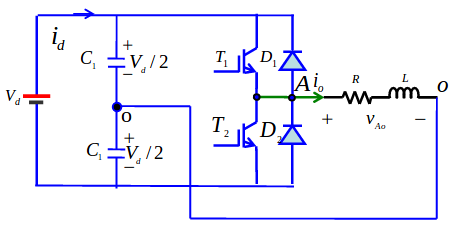
\includegraphics[width=0.07\textwidth]{PWMunipolar.png}
		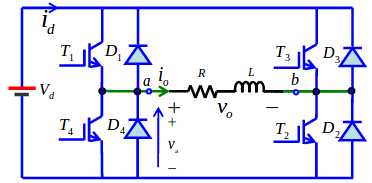
\includegraphics[width=0.07\textwidth]{PWMbipolar.png}
		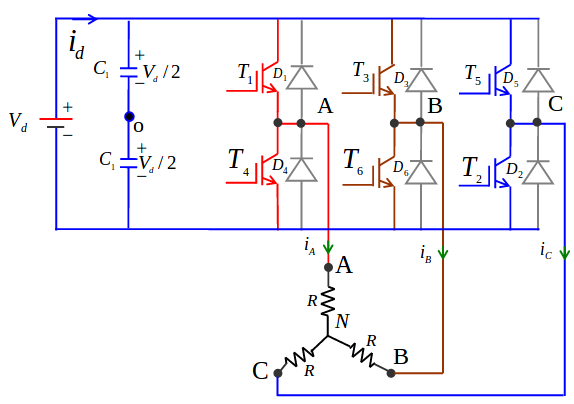
\includegraphics[width=0.07\textwidth]{PWM3phase.png}\\
		\textbf{Deadtime inverter:} avoids the shoot through during switch on/off that would result in a short circuit across the transistor bridge.\\
		\inlineimage{deadtime.png}
		
		
	\end{multicols*}
\end{document}